\documentclass[en]{../../../../../../eplexam}
\usepackage{../../../../../../eplcode}
\usepackage{todonotes}

\hypertitle{Concurrent Systems}{7}{INGI}{2143}{2020}{Janvier}{All}
{SINFO students 2019--2020}
{Charles Pecheur}

\section{Consider the following FSP model :}
\begin{lstlisting}
range Val = 0..(Nv-1)
range Addr = 0..(Na-1)

ADD = (	mem[a1:Addr].get[v1:Val] ->
		mem[a2:Addr].get[v2:Val] ->
		mem[a1].put[(v1+v2)%Nv] ->
		ADD).

ONE = (	mem[a1:Addr].put[1] -> ONE).

MEM = MEM1[0],
MEM1[v:Val] = (	get[v] -> MEM1[v]
				| put[v1:Val] ->MEM1[v1]).

||SYSTEM = ( add:ADD || one:ONE || {add,one}::mem[Val]:MEM).
\end{lstlisting}
\subsection{Draw the LTS of ADD for Na = 2, Nv=1}
\begin{solution}
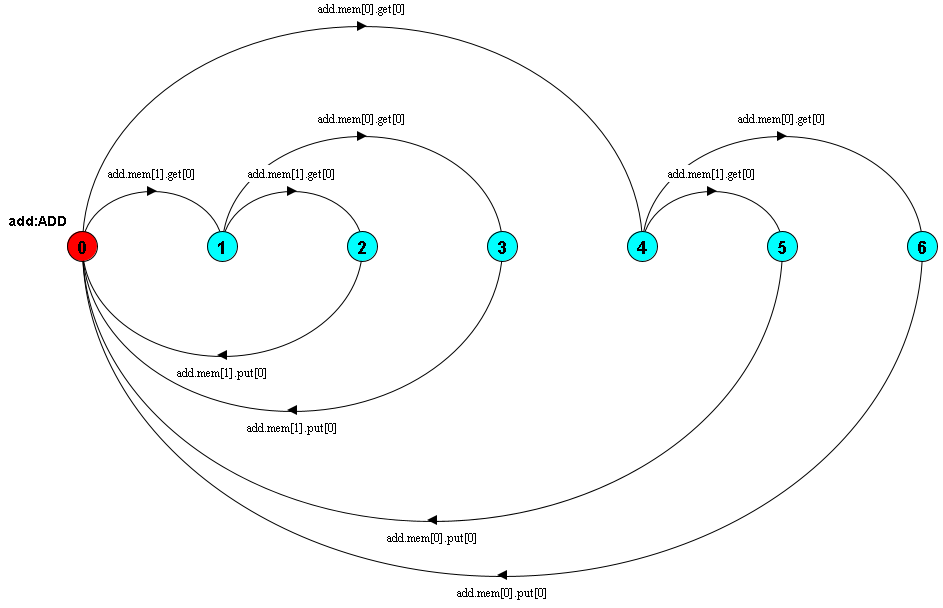
\includegraphics[width = \textwidth]{img/lts.png}
\end{solution}
\subsection{List the alphabet of SYSTEM in terms of Nv and Na (you may use range notations for conciseness).}
\begin{solution}
Solution for Na = 3 and Nv $\leq$ Na
\begin{verbatim}
{add, one}.mem[0..2].{get, put}[0..2]
\end{verbatim}
\end{solution}
\subsection{Let \#P be the number of states of P. Express \#ADD \#ONE \#MEM \#SYSTEM in terms of Nv and Na }
\begin{solution}

\noindent\#ADD = 1 + Na*Nv + (Na*Nv)$^2$

\noindent\#ONE = 1

\noindent\#MEM = Nv

\noindent\#SYSTEM = \#ADD * \#MEM$^{Na}$
\end{solution}
\subsection{Show an execution trace of SYSTEM for Nv=Na=3 containing the following actions : }
\begin{verbatim}
add.mem.0.get.1
add.mem.1.get.2
\end{verbatim}
\begin{solution}
\begin{verbatim}
one.mem.0.put.1
one.mem.1.put.1
one.mem.1.get.1
one.mem.0.get.1
one.mem.1.put.2
add.mem.0.get.1
add.mem.1.get.2
one.mem.0.put.0
\end{verbatim}
\end{solution}
\section{Consider the following FSP process definition:}
\begin{verbatim}
P1 = (a -> (c -> P1 | b -> c -> P1)).
P2 = (a -> c -> P2|a -> b -> c -> P2).
P3 = (a -> Q3),
Q3=(c -> P3|b -> c -> a -> Q3).
P4 = (a -> (b -> Q4|c -> P4)),
Q4 = (c -> a -> b -> P4).
\end{verbatim}
Which ines of P1,P2,P3,P4 are trace equivalent(TE), strongly bisimilar(SB), weakly bisimilar (WB) or not equivalent (NO) to each other?

\begin{solution}
\begin{itemize}
\todo[inline]{TODO : Complete solution}

	\item P1/P2 : % not WB
	\item P1/P3 : SB 
	\item P1/P4 : % not SB
	\item P2/P3 : TE
	\item P2/P4 : % not WB
	\item P3/P4 : % not SB
\end{itemize}
\end{solution}
\section{Assuming given fluents TIRED, EAT and SLEEP, specify the folowing properties in linear teemporal logic. Use parantheses to avoid ambiguity}
\begin{enumerate}
	\item You can never eat and sleep at the same time
	\item Whenever you are tired, you remain tired unless you sleep
	\item If you never eat, sooner or later you will sleep forever ( i.e. die)
	\item You are always tired immediately after eating
\end{enumerate}
\begin{solution}
	\begin{enumerate}
		\item \begin{verbatim}[]  ! (EAT && SLEEP)}\end{verbatim}
		\item \begin{verbatim}TIRED -> (TIRED W SLEEP)\end{verbatim}
		\item \begin{verbatim}(! EAT) -> <> [] SLEEP\end{verbatim}
		\item \begin{verbatim}EAT -> X TIRED\end{verbatim}
	\end{enumerate}
\end{solution}
\section{Consider the following Petri Net:}
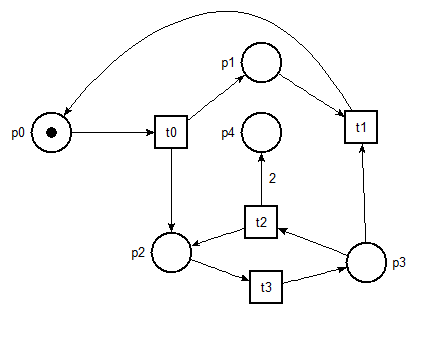
\includegraphics[width = 0.5\textwidth]{img/petri.png}
\subsection{List its place and transition invariants}
\begin{solution}
\begin{itemize}
	\item p0 p2 p3
	\item p0 p1
	\item t0 t1 t3
\end{itemize}
\end{solution}
\subsection{Construct its coverability tree}
\begin{solution}
\todo[inline]{TODO : Check if solution is correct}

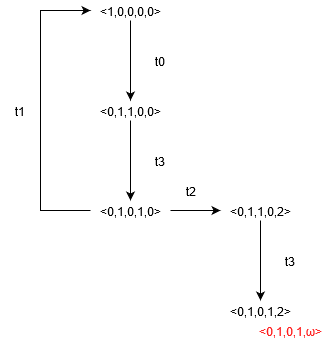
\includegraphics[width = 0.5\textwidth]{img/reach.png}
\end{solution}

\subsection{Which of the following markings for <p0,p1,p2,p3,p4> are reachable? Which ones are coverable?}
\begin{itemize}
	\item M1 = <0,1,0,1,2>
	\item M2 = <0,1,1,1,0>
	\item M3 = <0,1,1,0,5>
	\item M4 = <1,0,0,0,10>
\end{itemize}

\begin{solution}
\begin{itemize}
	\item M1 : reachable
	\item M2 : not coverable
	\item M3 : coverable
	\item M4 : reachable
\end{itemize}
\end{solution}


\end{document}
